
Skyline is a query operation that retrieves data items which are
considered ``interesting objects'' with respect to multiple
attributes of the data set. For example, someone who is planning
for an ocean-view vacation would be interested to find a list of
hotels that are close to the ocean and at the same time not too
expensive. A hypothetical data set of hotels is shown in
Table~\ref{tab:sample_data}. The two relevant attributes in this
case are \emph{minimum distance} to the ocean and \emph{minimum
price}. Figure~\ref{fig:skyline} shows the skyline points in solid
dots as the operation finds hotel records that are successively
further from the ocean, but the prices are the best for such
distances. In the figure, hotel $a$ is a skyline point because it
is closest to the ocean, although it is not the lowest price.
Hotels $b$ and $d$ are part of the skyline because each have the
closest distance at its price. Hotel $k$ is a skyline point
because it is the cheapest of all hotels.

\begin{figure}[h]
\centering \subfigure[2-D skyline of hotels of (X = min, Y = min)]{
    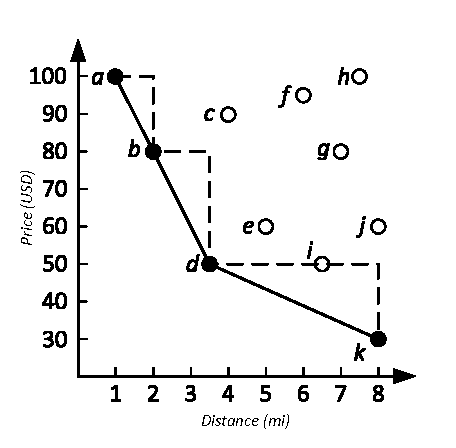
\includegraphics[width=1.5in]{Figures/skyline_points.eps}
    \label{fig:skyline}
} \subfigure[3-D skyline of stocks with attributes (X = min, Y = min, Z = max)]{
    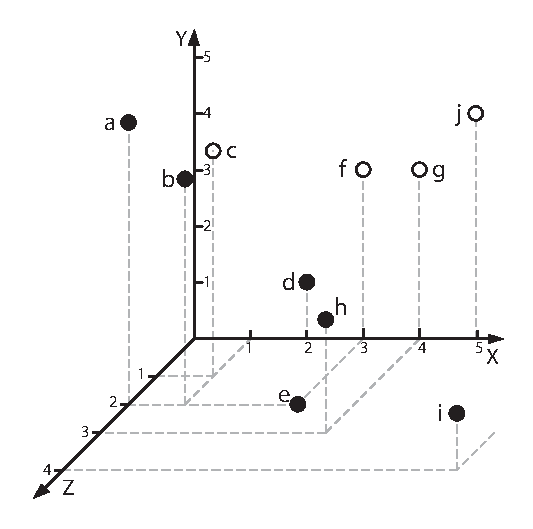
\includegraphics[width=1.5in]{Figures/skyline_points_3d.eps}
    \label{fig:skyline_points_3d}
} \caption{Sample Skylines}
\end{figure}

\begin{table}[b!]
  %\vspace*{-10pt}
  \centering
  \caption{Sample Data}
  %\vspace*{5pt}
  \label{tab:sample_data}
  \subfigure[\small 2-d Data of Fig 1(a)]{
  \label{tab:sample_data_a}
  \begin{tabular}{|c|c|c|}
  \hline
  {\bf Hotel} & {\bf Distance} & {\bf Price} \\ \hline\hline
  a & 1 & 8\\
  b & 2 & 6\\
  c & 4 & 7\\
  d & 3.5 & 3\\
  e & 5 & 4\\
  f & 6 & 7.5\\
  g & 7 & 6\\
  h & 7.5 & 8\\
  i & 6.5 & 3\\
  j & 8 & 4\\
  \hline
  \end{tabular}
  }
  \subfigure[\small 3-d data of Fig 1(b)]{
  \label{tab:sample_data_b}
  \begin{tabular}{|c|c|c|c|}
  \hline
  {\bf Symbol} & {\bf Price} & {\bf P/E} & {\bf Yield} \\ \hline\hline
  a & 0 & 5 & 2\\
  b & 1 & 4 & 2\\
  c & 1 & 4 & 1\\
  d & 2 & 2 & 0\\
  e & 3 & 0 & 2\\
  f & 3 & 3 & 0\\
  g & 4 & 3 & 0\\
  h & 4 & 2 & 3\\
  i & 7 & 1 & 4\\
  j & 5 & 4 & 0\\
  \hline
  \end{tabular}
  }
\end{table}


Skyline has broad applications and relevance due to multi-criteria
benefit. Skyline computation in realtime streaming systems with
frequent data updates has been studied in~\cite{Lin05stabbingthe}
and~\cite{Tao06maintainingsliding}. For distributed web services,
skyline query solutions have been proposed
in~\cite{Balke04efficientdistributed}. Skyline query has also been
applied in sensor networks
in~\cite{Seong:2009:ESQ:1644993.1645022}. Meanwhile, the data
broadcast is a scalable way to disseminate data (e.g., FM
broadcasting). Unlike the on-demand model, such as most of the
services on the Internet, the broadcast model can scale almost
indefinitely. A challenge and drawback of this model is the
forward-only access characteristic. While many studies have been
done on different query types to support efficient query
evaluation in broadcast
environments~\cite{DBLP:journals/tmc/KuZW08,dsi,DBLP:conf/cikm/Hara02},
to the best of our knowledge, the work
in~\cite{Ha:2009:EEP:1616994.1617050} is the only study on skyline
query processing in broadcast environments.
Although~\cite{Ha:2009:EEP:1616994.1617050} considers broadcast
efficiency (more details in Section~\ref{sec:wireless_broadcast}),
the proposed solution is unable to support all possible skyline
types (i.e., combinations of min and max attributes) and the work
did not address skyline of higher data dimension ($>2$ dimensions)
as illustrated in figure~\ref{fig:skyline_points_3d}. To address
these challenges, we design a flexible broadcast index and a
skyline evaluation algorithm that utilizes the index to
efficiently evaluate skyline queries. Specifically, our
contributions of this research are as follows:

%In broadcast environment, the clients listens on the broadcast for data records and evaluates
%the skyline queries from the records. The challenge is the forward only data model. A goal
%of this research is to incorporate necessary structure in the broadcast data to help client
%prune unnecessary data.

%While many studies have been done on efficiently evaluating skyline operation in traditional
%database systems, in the best of our knowledge, only one study has been done on skyline
%evaluation in broadcast system. \cite{Ha:2009:EEP:1616994.1617050} proposed encoding
%the data records using Sweep space-filling curve (SFC) over relevant attributes before
%broadcasting the system.
%as shown in Figure \ref{fig:SFC}.
%Since the encoding process decides
%a specific skyline application,
%such that the encoding can be used for the MINIMUM skyline operation on all attributes, such
%encoding and broadcast is not flexible to support different kinds of application from the
%broadcast program. In addition SFC encoding is inflexible in data with more than two dimensions.

%In this paper, we propose a flexible technique for evaluation of skyline in broadcast environment.
%Our technique is a general indexing technique that can easily incorporate different index structures,
%such as the R-Tree and the KD-Tree\cite{Bentley:1975:MBS:361002.361007}, into the index structure
%to facilitate evaluation on broadcast
%program. An advantage of this flexibility is that for data of high dimension, the system can use
%KD-Tree, while data of low dimension (two or three), R-Tree can be an efficient choice. Our solution
%is based on pruning region concept and does not restrict the skyline operation to either MAX or
%MIN. The client is able to choose between these two criteria on any of the attributes of the data.

\begin{itemize}
\item We design a flexible on air index that supports skyline
query evaluation in data broadcast environments for arbitrary
number of data dimension.

\item We propose an efficient data broadcast skyline query
algorithm that handles both min and max attributes.

\item We evaluate the performance of the proposed algorithms
through extensive experiments.
\end{itemize}

The rest of this paper is organized as follows. Section 2 provides
background knowledge of the skyline operator and wireless data
broadcast. We introduce our index structures to facilitate
broadcast skyline query in Section 3. In Section 4 we propose our
pruning region based technique for skyline query evaluation. The
experimental validation of our design is presented in Section 5.
Section 6 surveys related works. We conclude the paper with a
discussion of future work in Section 7.
